%//////////////////////////////////
%/// P R E A M B L E

\documentclass[a4paper, 12pt]{article}

\usepackage[utf8]{inputenc}
\usepackage[singlespacing]{setspace}
\usepackage{amsmath}
\usepackage{mathtools}
\usepackage{caption}
\usepackage{float}
\usepackage{booktabs}
\usepackage{graphicx}
\usepackage{multicol}
\usepackage{gensymb}
\usepackage{breqn}
\usepackage{indentfirst}
\usepackage{siunitx}
\usepackage{tabularx, booktabs}
\newcolumntype{Y}{>{\centering\arraybackslash}X}

\usepackage{pdfpages}

\usepackage{multicol}
\usepackage{supertabular}

\usepackage{svg}

\widowpenalty = 4500
\clubpenalty  = 4500

\setlength{\jot}{10pt} %indents


\newcommand*\dif{\mathop{}\!\mathrm{d}}
\newcommand*\shortminus{\scalebox{0.5}[1.0]{\( - \)}}
%\newcommand{\euler}{\mathrm{e}}
%\newcommand{\ramuno}{\mathrm{j}}

%%========================================
%% circuitikz properties
\usepackage[european, straightvoltages]{circuitikz}
%\ctikzvalof{voltage/distance from node = .2}
%\ctikzset{voltage/distance from node  =.5}% in \pgf@circ@Rlen units
%\ctikzset{voltage/distance from line  =.25}% pos. between 0 and 1
%\ctikzset{voltage/bump b/.initial     =1.5}%

\ctikzset{current/distance            = .618}


%%========================================

%%
%% Path settings
%%
\graphicspath{ {./graphics/} }


%//////////////////////////////////
%/// D O C U M E N T
\begin{document}

%%%%%%%%%%%%%%%%%%%%%%%%%%%%%%%%%%%%%
  \includepdf{Deckblatt.pdf}
  
\includepdf{./titlepage/titlepage.pdf}
%%%%%%%%%%%%%%%%%%%%%%%%%%%%%%%%%%%%%

\section{Vorbereitungsaufgaben}

  % 2.1
  \subsection{}
    \begin{center}
      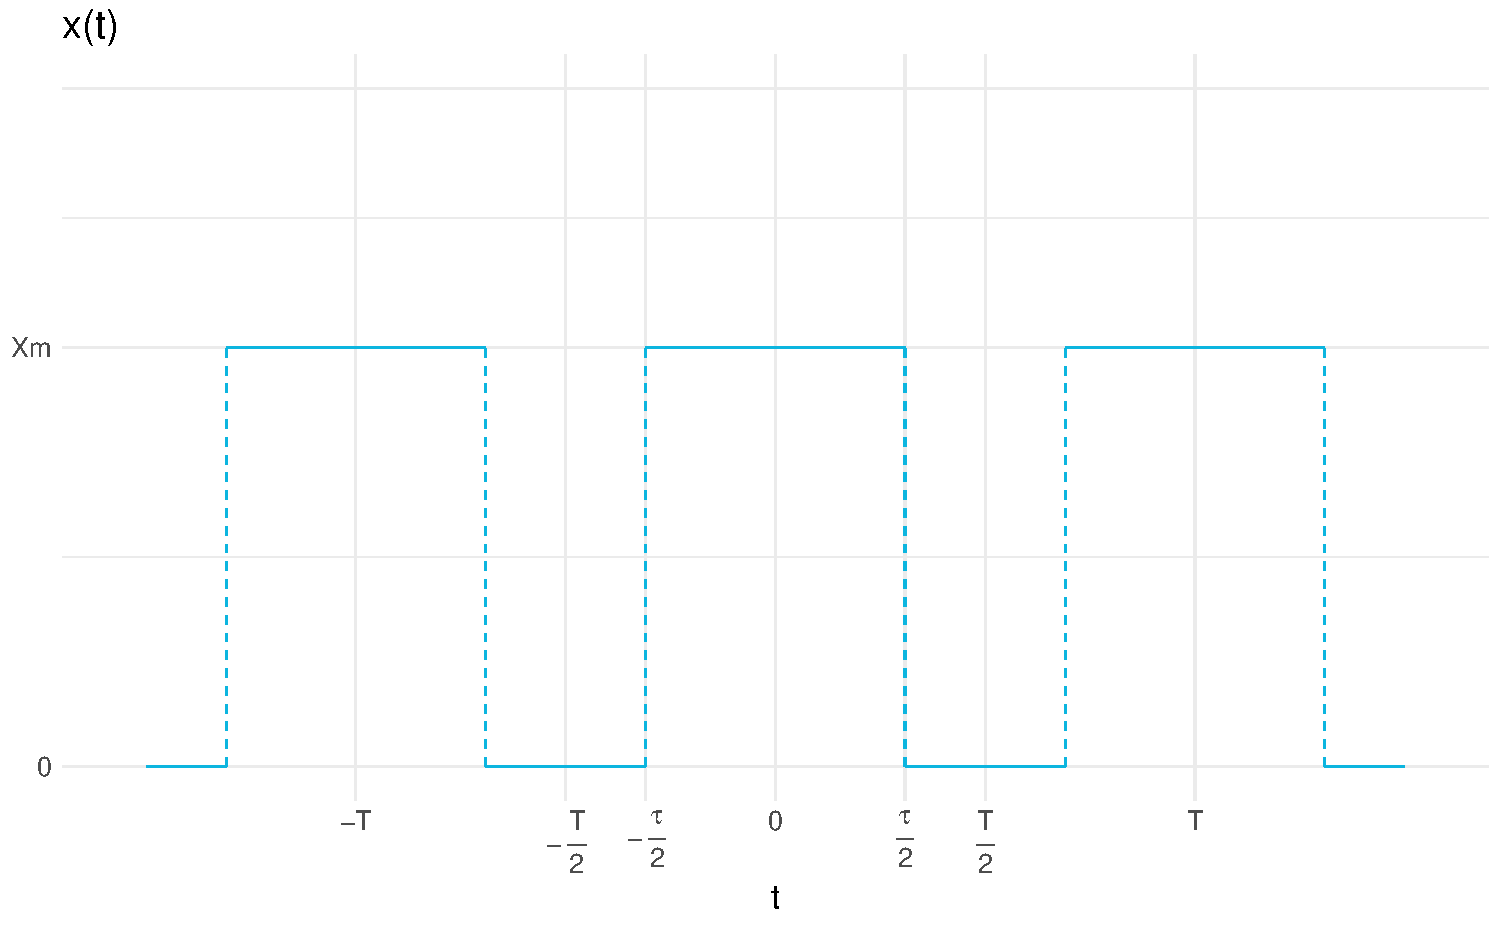
\includegraphics[scale=0.5]{./R/2_1/2_1_function.pdf}
    \end{center}

    \begin{align*}
      \underline{X}_\nu &= \frac{1}{T_1} \cdot \int_{T_1}{x(t) \cdot e^{-(j\nu\cdot\omega_1t)}\dif t}\\
      &= \frac{1}{T_1} \cdot \int_{\shortminus\frac{\tau}{2}}^{\frac{\tau}{2}}{ X_m \cdot e^{-(j\nu\cdot\omega_1t)}\dif t}\\
      &= - \frac{X_m}{T_1 \cdot j \nu \omega_1 } \cdot \left[  e^{-(j\nu\cdot\omega_1t)} \right]^{\frac{\tau}{2}}_{\shortminus\frac{\tau}{2}}\\
      &= -\frac{X_m}{T_1 \cdot j \nu \omega_1 } \cdot \left ( e^{-j\nu\cdot\omega_1 \frac{\tau}{2}} - e^{j\nu\cdot\omega_1 \frac{\tau}{2}} \right )
      %
      \intertext{$\omega_1 = \frac{2 \pi}{T_1}$ und Erweiterung mit $\frac{-1}{-1}$:}
      \underline{X}_\nu &= \frac{X_m}{2 j \pi \nu } \cdot \left ( e^{j\nu\cdot \pi \frac{\tau}{T_1}} - e^{-j\nu\cdot \pi \frac{\tau}{T_1}} \right )\\
      &= \frac{X_m}{\pi \nu } \cdot \frac{\left ( e^{j\nu\cdot \pi \frac{\tau}{T_1}} - e^{-j\nu\cdot \pi \frac{\tau}{T_1}} \right )}{2 j}
    \end{align*}

    \begin{gather*}
      \text{\small{ mit $ \frac{\left ( e^{jx} - e^{-jx} \right )}{2 j} = \sin{(x)}$ und $\frac{\tau}{T_1} = D$: }}\notag\\
      \underline{X}_\nu = \frac{X_m}{\pi \nu } \cdot \sin{(\pi \nu D)}
    \end{gather*}

    \begin{gather*}
        \text{\small Erweitert man wieder mit $\frac{D}{D}$ erhält man das Bild einer Spaltfunktion $\text{si}(x)=\frac{\sin x }{x}$: }\notag\\
        \underline{X}_\nu = D \cdot X_m \cdot \frac{\sin(\pi \nu D)}{\pi \nu D} = D \cdot X_m \cdot \text{si}(\pi \nu D)
      %\shortintertext{or}
    \end{gather*}

    \begin{gather*}
        \text{\small Als reele Reihe:}\notag\\
        x(t) = X_0 + \sum^{\infty}_{\nu=1}{\hat{X}_\nu \cos(\nu \cdot \omega_1 t + \phi_\nu )}\\
        X_0 = \frac{1}{T_1} \cdot \int_{T_1}{x(t) \dif t} = \frac{X_m}{2}\\
    \end{gather*}

    \begin{gather*}
      \text{\small Aus der komplexen Reihendarstellung folgt}\notag\\
      b_\nu = -2 \cdot \text{Im}(\underline{X}_\nu) = 0\\
      \hat{X}_\nu = \sqrt{a^2_\nu + b^2_\nu} = 2 \cdot \mid \underline{X}_\nu\mid \implies a_\nu = 2 \cdot \mid D \cdot X_m \cdot \text{si}(\nu \pi D)\mid \\
      \text{\small $\phi_\nu$ hängt nur vom Wert von $\text{si}{(\nu \pi D)}$ ab, da $\underline{X}_\nu$ rein reell ist:}\notag\\
      \phi_\nu =
      \begin{dcases}
      0 & ; \nu = \frac{4k+1}{2D} \\
      \pi & ; \nu =\frac{4k-1}{2D} \\
      \text{n.d.} & ; \text{sonst}
      \end{dcases}
      %\text{\small also}\notag\\
      %a_\nu = \hat{X}_\nu, \,\
      %\phi_\nu = 0
    \end{gather*}

    \begin{gather*}
      \text{\small Somit ist}\notag\\
      x(t) = \frac{X_m}{2} + \sum^{\infty}_{\nu=1}{2 D X_m \cdot \mid \text{si}(\pi \nu D) \mid \cdot \cos(\nu \cdot \frac{2\pi}{T_1} \cdot t + \phi_\nu)}
    \end{gather*}

    \vspace{0.021276873\paperheight}

    \begin{center}
      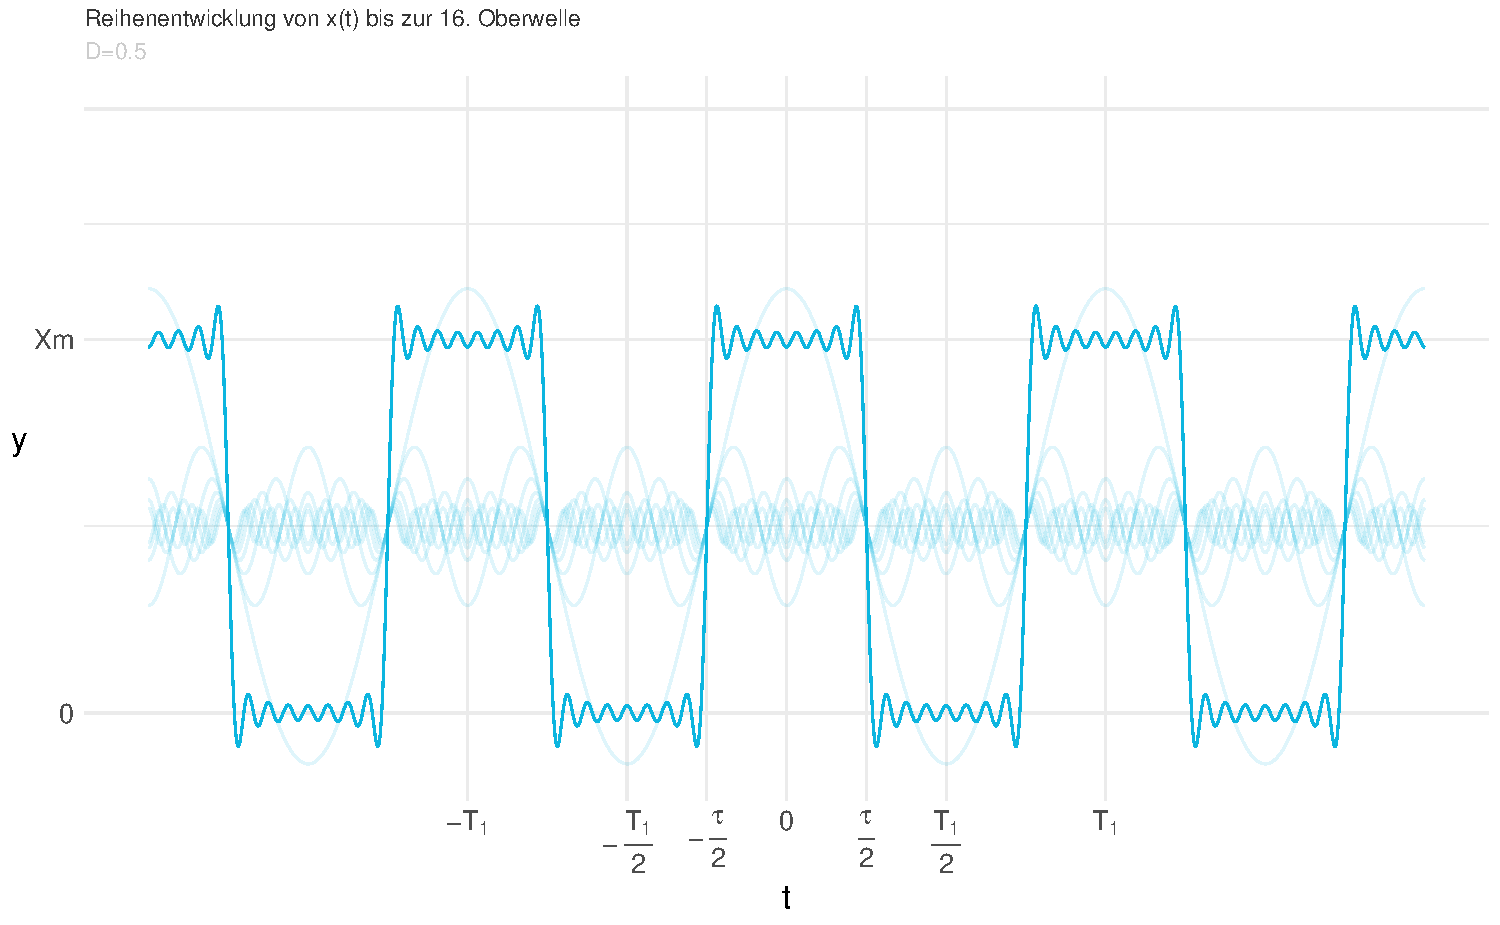
\includegraphics[scale=0.5]{./R/2_1/2_1_Reihe.pdf}
    \end{center}

    \begin{gather*}
      \text{\small Effektivwert:}\notag\\
      X_{\text{eff}} = \sqrt{ \frac{1}{T_1} \cdot \int_{T_1}{x^2(t) \dif t} } = \sqrt{ \frac{X_m^2}{T_1} \cdot \int_{\shortminus\frac{\tau}{2}}^{\frac{\tau}{2}}{1 \dif t} }\\
      X_{\text{eff}}= X_m \cdot \sqrt{\frac{\tau}{T_1}} = X_m \cdot \sqrt{D}
    \end{gather*}

    %\vspace{0.021276873\paperheight}

    \begin{center}
      \bgroup
      \def\arraystretch{1.6180339887498948}
        \begin{tabular}{@{}cccc@{}}
        \toprule
        \multicolumn{3}{c}{$D = \frac{1}{2}, X_{\text{eff}}=\frac{X_m}{\sqrt{2}}$} \\ \midrule
        $\nu$      & $\underline{X}_\nu$   & $\hat{X}_\nu$ & $\phi_\nu$ \\ \hline
        1          &  $\frac{1}{\pi} X_m$      &      $\frac{2}{\pi} X_m$&        $0$\\
        2          &  $-$         &       $-$      & $-$  \\
        3          &  $\shortminus\frac{1}{3\pi} X_m$         &   $\frac{2}{3\pi} X_m$   &        $\pi$\\
        4          &  $-$         &       $-$    &$-$    \\
        5          &  $\frac{1}{5\pi} X_m$      &       $\frac{2}{5\pi} X_m$    &  $0$ \\
        6          &  $-$         &       $-$    & $-$   \\
        7          &  $\shortminus\frac{1}{7\pi} X_m$         &          $\frac{2}{7\pi}X_m$  & $\pi$\\
        8          &  $-$         &       $-$     & $-$   \\
        9          &  $\frac{1}{9\pi} X_m$         &       $\frac{2}{9\pi} X_m$   &  $0$   \\
        10         &  $-$         &       $-$       & $-$ \\
        11         &  $\shortminus\frac{1}{11\pi} X_m$         &       $\frac{2}{11\pi} X_m$  &   $\pi$ \\
        12         &  $-$         &       $-$      & $-$  \\
        13         &  $\frac{1}{13\pi} X_m$         &      $\frac{2}{13\pi} X_m$ &   $0$   \\
        14         &  $-$         &      $-$       & $-$  \\
        15         &  $\shortminus\frac{1}{15\pi} X_m$         &      $\frac{2}{15\pi} X_m$   &  $\pi$  \\
        16         &  $-$         &       $-$      & $-$  \\ \bottomrule
        \end{tabular}
        \hspace{0.6180339887498948cm}
        \begin{tabular}{@{}ccc@{}}
        \toprule
        \multicolumn{3}{c}{$D = \frac{1}{4}, X_{\text{eff}}=\frac{X_m}{2}$} \\ \midrule
        $\nu$      & $\hat{X}_\nu$   & $\phi_\nu$ \\ \hline
        1          &  $\frac{\sqrt{2}}{\pi} X_m$      &      $0$        \\
        2          &  $\frac{1}{\pi} X_m$         &       $0$        \\
        3          &  $\frac{\sqrt{2}}{3\pi} X_m$         &   $0$           \\
        4          &  $-$         &       $-$        \\
        5          &  $\frac{\sqrt{2}}{5\pi} X_m$      &       $\pi$      \\
        6          &  $\frac{1}{3\pi} X_m$         &       $\pi$      \\
        7          &  $\frac{\sqrt{2}}{7\pi} X_m$         &          $\pi$   \\
        8          &  $-$         &       $-$       \\
        9          &  $\frac{\sqrt{2}}{9\pi} X_m$         &       $0$      \\
        10         &  $\frac{1}{5\pi} X_m$         &       $0$       \\
        11         &  $\frac{\sqrt{2}}{11\pi} X_m$         &       $0$      \\
        12         &  $-$         &       $-$       \\
        13         &  $\frac{\sqrt{2}}{13 \pi} X_m$         &      $\pi$       \\
        14         &  $\frac{1}{7\pi} X_m$         &      $\pi$        \\
        15         &  $\frac{\sqrt{2}}{15\pi} X_m$         &      $\pi$       \\
        16         &  $-$         &       $-$       \\ \bottomrule
        \end{tabular}
        \hspace{0.6180339887498948cm}
        \begin{tabular}{@{}ccc@{}}
        \toprule
        \multicolumn{3}{c}{$D = \frac{1}{8}, X_{\text{eff}}=\frac{X_m}{\sqrt{8}}$} \\ \midrule
        $\nu$      & $\hat{X}_\nu$   & $\phi_\nu$ \\ \hline
        1          &  $\frac{\sqrt{2-\sqrt{2}}}{\pi} X_m$      &      $0$        \\
        2          &  $\frac{\sqrt{2}}{2\pi}X_m$         &       $0$        \\
        3          &  $\frac{\sqrt{2 + \sqrt{2}}}{3\pi}X_m$         &   $0$           \\
        4          &  $\frac{1}{2}X_m$         &       $0$        \\
        5          &  $\frac{\sqrt{2 + \sqrt{2}}}{5\pi}X_m$      &       $0$      \\
        6          &  $\frac{\sqrt{2}}{16\pi}X_m$         &       $0$      \\
        7          &  $\frac{\sqrt{2 - \sqrt{2}}}{7\pi}X_m$         &          $0$   \\
        8          &  $-$         &       $-$       \\
        9          &  $\frac{\sqrt{2 - \sqrt{2}}}{9\pi}X_m$         &       $\pi$      \\
        10         &  $\frac{\sqrt{2}}{5\pi}X_m$         &       $\pi$       \\
        11         &  $\frac{\sqrt{2 + \sqrt{2}}}{11\pi}X_m$         &       $\pi$      \\
        12         &  $\frac{1}{6\pi}X_m$         &       $\pi$       \\
        13         &  $\frac{\sqrt{2 + \sqrt{2}}}{13\pi}X_m$         &      $\pi$       \\
        14         &  $\frac{\sqrt{2}}{7\pi}X_m$         &      $\pi$        \\
        15         &  $\frac{\sqrt{2 - \sqrt{2}}}{15\pi}X_m$         &      $\pi$       \\
        16         &  $-$         &       $-$       \\ \bottomrule
        \end{tabular}
        \egroup
      \end{center}

  % 2.2
  \subsection{}
    \begin{center}
      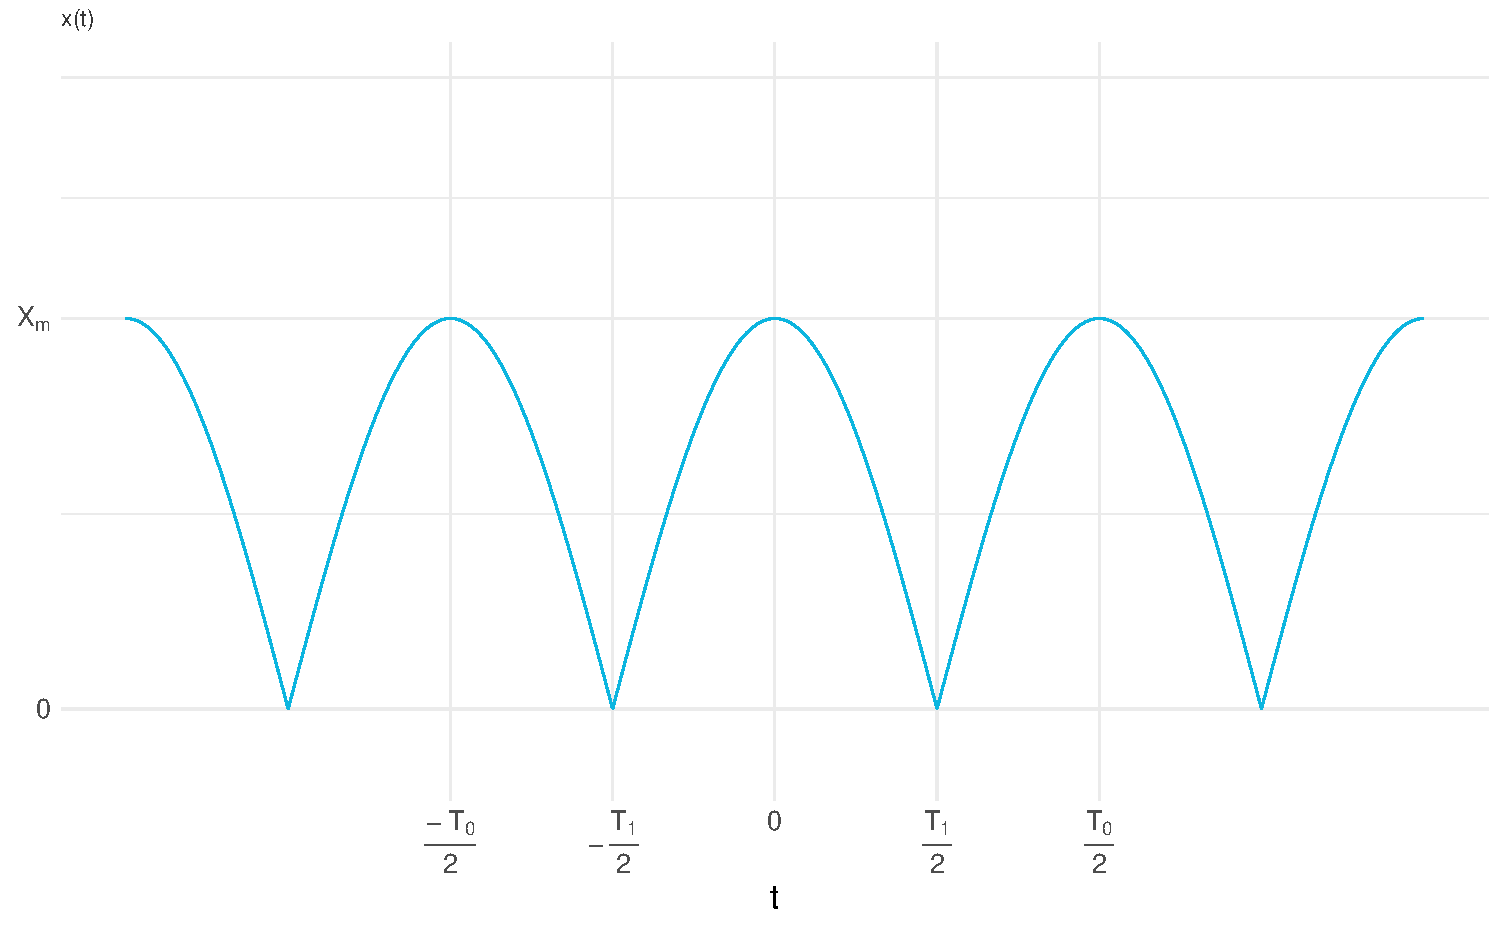
\includegraphics[scale=0.5]{./R/2_2/2_2_function.pdf}
    \end{center}

    \begin{align*}
      \underline{X}_\nu &= \frac{1}{T_1} \cdot \int_{\shortminus\frac{T_1}{2}}^{\frac{T_1}{2}}{ X_m \cos{(\frac{\pi}{T_1} t) \cdot e^{-(j\nu \frac{\pi}{T_1} t)}} \dif t }\\
      &= \frac{X_m}{T_1} \cdot \left [ \frac{e^{-(j\nu \frac{\pi}{T_1} t)}}{(-j \nu \frac{\pi}{T_1})^2+(\frac{\pi}{T_1})^2} \cdot \left( (-j\nu\frac{\pi}{T_1})\cdot \cos{(\frac{\pi}{T_1} t )} + \frac{\pi}{T_1}\cdot \sin{(\frac{\pi}{T_1} t)} \right) \right]_{\shortminus\frac{T_1}{2}}^{\frac{T_1}{2}}\\
      &= \frac{X_m}{\pi (1-4\nu^2)} \cdot \left[  e^{-j\nu\pi} \cdot (\underbrace{-j 2 \nu \cdot \cos{(\frac{\pi}{2})}}_0+1) - e^{j\nu\pi} \cdot (\underbrace{-j 2 \nu \cdot \cos{(-\frac{\pi}{2})}}_0-1) \right]\\
      &= \frac{X_m}{\pi (1-4\nu^2)} \cdot (e^{-j\nu\pi}+e^{j\nu\pi}) = 2 \frac{X_m}{\pi (1-4\nu^2)} \cdot \left( \frac{e^{j\nu\pi}+e^{-j\nu\pi}}{2} \right)
    \end{align*}

    \vspace{0.021276873\paperheight}
    \begin{equation*}
      \underline{X}_\nu =  \frac{2 X_m}{\pi (1-4\nu^2)} \cdot \cos{(\nu \pi)}
    \end{equation*}

    \begin{gather*}
      \hat{X}_\nu = 2 \cdot \mid \underline{X}_\nu \mid = \frac{4 \cdot X_m}{\pi (1-4\nu^2)}\cdot \cos{(\nu \pi)}
    \end{gather*}
    \begin{gather*}
      \text{\small Mittelwert:}\\
      X_0 = \frac{1}{T_1} \cdot \int_{\shortminus\frac{T_1}{2}}^{\frac{T_1}{2}}{X_m \cdot \cos{(\frac{\pi}{T_1} t)} \dif t} = \frac{X_m}{\pi} \cdot \left[\sin{(\frac{\pi}{T_1}t)} \right]_{\shortminus\frac{T_1}{2}}^{\frac{T_1}{2}}\\
      X_0 = \frac{2 X_m}{\pi}
    \end{gather*}

    \begin{gather*}
      \text{\small Effektivwert:}\\
      X_{\text{eff}} = \sqrt{\frac{X_m^2}{T_1} \cdot \int_{\shortminus\frac{T_1}{2}}^{\frac{T_1}{2}}{(\cos{(\frac{\pi}{T_1} t))^2} \dif t}}\\
      X_{\text{eff}} = \sqrt{ \frac{X_m^2}{T_1} \cdot \left[  \frac{t}{2} + \frac{\sin{(\frac{2\pi}{T_1})t}}{4 \cdot \frac{\pi}{T_1}} \right]_{\shortminus\frac{T_1}{2}}^{\frac{T_1}{2}} }\\
      X_{\text{eff}} = \frac{X_m}{\sqrt{2}}
    \end{gather*}

    \begin{center}
      \bgroup
      \def\arraystretch{1.31}
      \begin{tabular}{@{}ccc@{}}
      \toprule
      \multicolumn{3}{c}{$D = \frac{1}{4}, X_{\text{eff}}=\frac{X_m}{2}$} \\ \midrule
      $\nu$      & $\hat{X}_\nu$   & $\phi_\nu$ \\ \hline
      1          &  $\frac{4}{3\pi} X_m$      &      $0$        \\
      2          &  $\frac{4}{15\pi} X_m$         &       $\pi$        \\
      3          &  $\frac{4}{35\pi} X_m$         &   $0$           \\
      4          &  $\frac{4}{63\pi} X_m$         &       $\pi$        \\
      5          &  $\frac{4}{99\pi} X_m$      &       $0$      \\
      6          &  $\frac{4}{143\pi} X_m$         &       $\pi$      \\
      7          &  $\frac{4}{195\pi} X_m$         &          $0$   \\
      8          &  $\frac{4}{255\pi} X_m$         &       $\pi$       \\
      9          &  $\frac{4}{323\pi} X_m$         &       $0$      \\
      10         &  $\frac{4}{399\pi} X_m$         &       $\pi$       \\
      11         &  $\frac{4}{483\pi} X_m$         &       $0$      \\
      12         &  $\frac{4}{575\pi} X_m$         &       $\pi$       \\
      13         &  $\frac{4}{675\pi} X_m$         &      $0$       \\
      14         &  $\frac{4}{783\pi} X_m$         &      $\pi$        \\
      15         &  $\frac{4}{899\pi} X_m$         &      $0$       \\ \bottomrule
      \end{tabular}
      \hspace{0.6180339887498948cm}
      \egroup
    \end{center}
    \vspace{0.021276873\paperheight}


  % 2.3
  \subsection{}
    \begin{center}
      \begin{circuitikz}

        \draw (0,0) to[V, v=$u_0(t)$] (0,-3);
        \draw (0,0) to[R, l=$R_1$, ] (5,0);
        %\draw (2,0) to[L, l=$L$, i=$\underline{I}$] (6,0);
        \draw (5,0) to[C, l=$C$, *-*] (5,-3);
        \draw (7,0) to[C, l=$R_2$, *-*] (7,-3);
        \draw (0,-3) to[short] (9.25,-3);
        \draw (5,0) to[short] (9.25,0);
        \draw (9.25,0) to[open, v^=$u_2(t)$, o-o] (9.25,-3);

      \end{circuitikz}
    \end{center}

    \begin{gather*}
      \underline{U}_2 = \underline{U_0} \cdot \dfrac{ \frac{1}{ j \omega C + \frac{1}{R_2} }  }{ R_1 + \frac{1}{ j \omega C + \frac{1}{R_2} } } = \frac{\underline{U}_0 \cdot R_2}{R_1+R_2+ j \omega C R_1 R_2}\\
      \text{\small Betrag:}\\
      \hat{U}_2 = \frac{\hat{U}_0 \cdot R_2}{\sqrt{(R_1+R_2)^2 + (\omega C R_1 R_2)^2}}\\\\
      \text{\small Phase:}\\
      \phi_{\underline{U}_2} = \phi_{\underline{U}_0} - \arctan{ \frac{\omega C R_1 R_2}{R_1+R_2} }\\\\
      \text{\small Mittelwert:}\\
      \underline{U}_{0_\nu} (\nu = 0) = \hat{U}_{0_\nu}(\nu=0) \cdot \frac{R_2}{R_1+R_2} = \frac{2 \cdot 1 \si{\volt}\cdot 1\si{\kilo\ohm}}{\pi\cdot(1\si{\kilo\ohm}+400\si{\kilo\ohm})} \approx 0.424 \,\ \si{\volt}
    \end{gather*}


      \begin{table}[H]
        \begin{center}
        \begin{tabular}{@{}ccccccc@{}}
        \toprule
        $\nu$ & $\underline{U}_{0_\nu} / \si{\volt}$ & $\hat{U}_{0_\nu}/ \si{\volt}$ & $\phi$ & $\hat{U}_{2_\nu}/ \si{\volt}$ & $\phi_{U_{2_\nu}}/ \si{\degree}$ & $U_{2_{\text{eff}}}/ \si{\volt}$ \\ \midrule
                1     & 0.2122                              & -0.4244                       & 0      &        0.1219                        & -60.88                           &       0.0862                           \\
        2     & -0.4244                             & 0.08488                       & $\pi$  &               0.0131               & 105.56                           &              0.0093                    \\
        3     & 0.0182                              & 0.03638                       & 0      &               0.0038          & -79.48                           &               0.0027                   \\
        4     & -0.0101                             & 0.02021                       & $\pi$  &               0.0016                & 97.93                            &              0.0011                    \\
        5     & 0.0064                              & 0.01286                       & 0      &               0.0008                & -83.64                           &               0.0006                   \\
        6     & -0.0045                             & 0.00890                       & $\pi$  &               0.0005                & 95.3                             &              0.0004                    \\
        7     & 0.0033                              & 0.00652                       & 0      &               0.0003                & -85.45                           &               0.0002                   \\
        8     & -0.0025                             & 0.00499                       & $\pi$  &               0.0002                & 93.19                            &              0.0001                    \\
        9     & 0.0020                              & 0.00394                       & 0      &                 -              & -86.45                           &                -                  \\
        10    & -0.0016                             & 0.00319                       & $\pi$  &                 -              & 93.19                            &              -                    \\
        11    & 0.0013                              & 0.00264                       & 0      &                 -              & -87.1                            &                -                  \\
        12    & -0.0011                             & 0.00221                       & $\pi$  &                 -              & 92.28                            &               -                   \\
        13    & -0.0009                             & 0.00189                       & 0      &                 -              & -87.55                           &               -                   \\
        14    & -0.0008                             & 0.00163                       & $\pi$  &                 -              & 92.28                            &               -                   \\
        15    & 0.0007                              & 0.00142                       & 0      &                 -              & -87.87                           &                -                  \\
        16    & -0.0006                             & 0.0012                        & $\pi$  &                  -             & 91.99                            &               -                   \\ \bottomrule
        \end{tabular}
        \end{center}
        \end{table}

      \begin{gather*}
        \text{\small Effektivwert aus Summe der einzelnen Effektivwerte:}\\
        U_{2_{\text{eff}}} = \sqrt{ U_{2_\nu}^2 + \sum_{\nu=1}^{\infty}{U_{2_{{\text{eff}}_\nu}}^2}} \approx 0.433 \,\ \si{\volt}
      \end{gather*}

    \vspace{0.021276873\paperheight}
    \begin{center}
      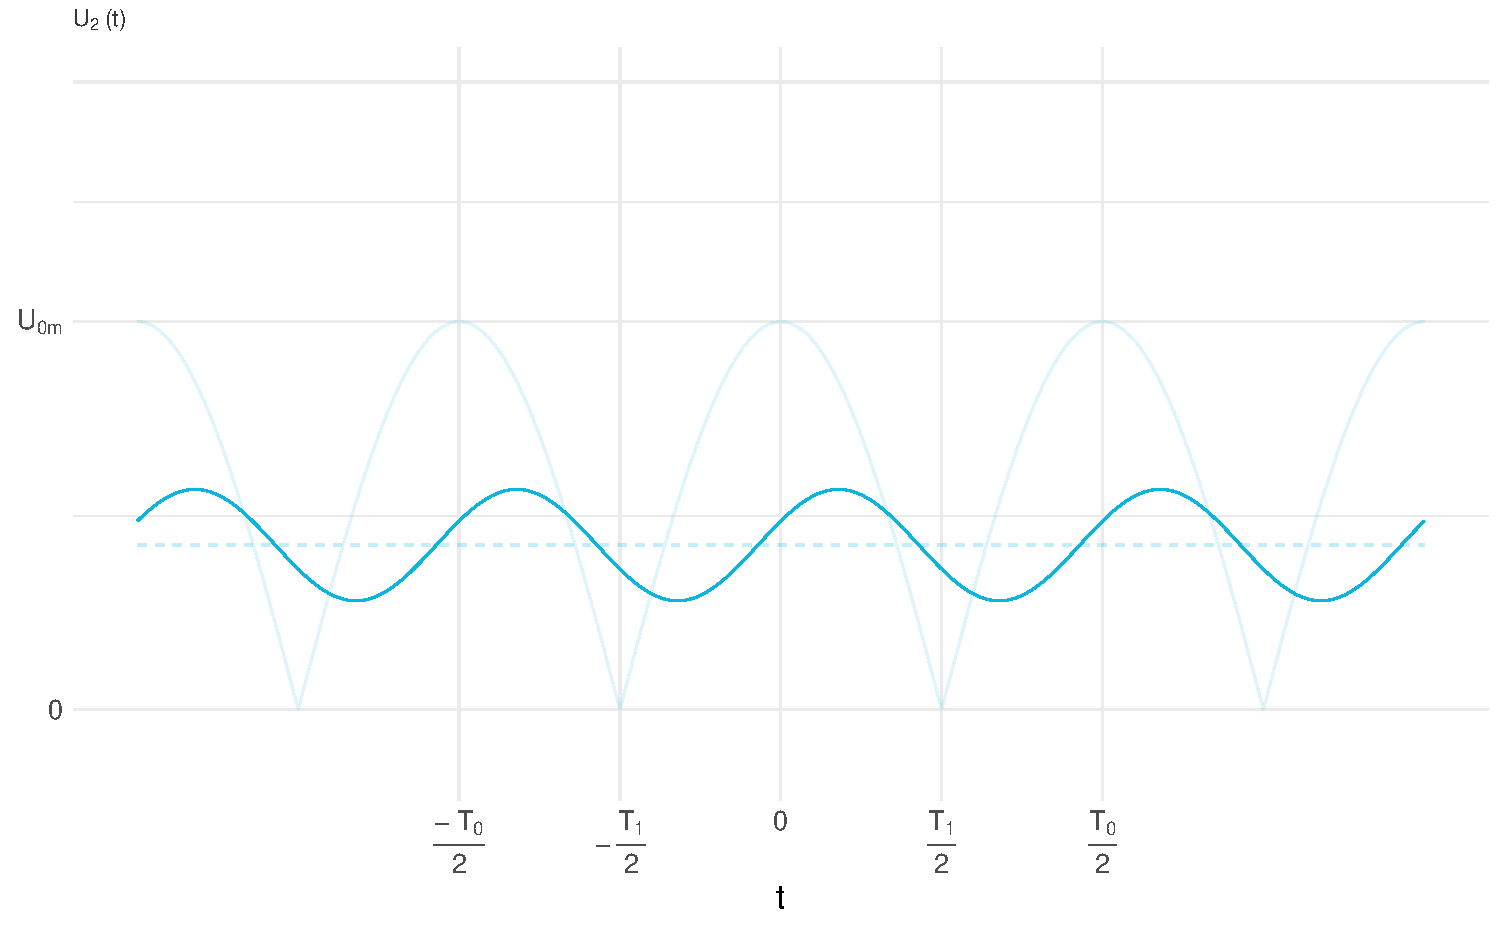
\includegraphics[scale=0.5]{./R/2_3/2_3_function.pdf}
    \end{center}



\pagebreak
\section{Versuchsaufgaben}
  % 3.1
  \subsection{}
  \begin{center}
    Messwerte der Aufgabe 3.1 für \emph{$T=10 \,\ \si{\micro\second}$}:\\
    \vspace{0.021276873\paperheight}
    \bgroup
    \def\arraystretch{1.6180339887498948}
      \begin{tabular}{@{}cccc@{}}
      \toprule
      \multicolumn{3}{c}{$D = \frac{1}{2}, X_{\text{eff}}=?$} \\ \midrule
      $\nu$      & $\hat{X}_\nu / \si{\milli\volt}$   & $X_{\nu_{\text{eff}}} / \si{\milli\volt}$ & $f_\nu / \si{\kilo\hertz}$ \\ \hline
        1     & 608.112                          & 430                                     & 100                        \\
        2     & -                                & -                                       & -                          \\
        3     & 208.045                          & 147.11                                  & 300                        \\
        4     & -                                & -                                       & -                          \\
        5     & 123.546                          & 87.36                                   & 500                        \\
        6     & -                                & -                                       & -                          \\
        7     & 91.040                           & 64.375                                  & 700                        \\
        8     & -                                & -                                       & -                          \\
        9     & 68.059                           & 48.125                                  & 900                        \\
        10    & -                                & -                                       & -                          \\
        11    & 57.544                           & 40.69                                   & 1100                       \\
        12    & -                                & -                                       & -                          \\
        13    & 48.691                           & 34.43                                   & 1300                       \\
        14    & -                                & -                                       & -                          \\
        15    & 41.606                           & 29.42                                   & 1500                       \\ \bottomrule
      \end{tabular}
      \egroup

      \bgroup
      \def\arraystretch{1.6180339887498948}
        \begin{tabular}{@{}cccc@{}}
        \toprule
        \multicolumn{3}{c}{$D = \frac{1}{4}, X_{\text{eff}}=500 \,\ \si{\milli\volt}$} \\ \midrule
        $\nu$      & $\hat{X}_\nu / \si{\milli\volt}$   & $X_{\nu_{\text{eff}}} / \si{\milli\volt}$ & $f_\nu / \si{\kilo\hertz}$ \\ \hline
        1  & 445.477     & 315        & 100      \\
        2  & 311.070     & 219.96     & 200      \\
        3  & 143.401     & 101.4      & 300      \\
        4  & -            & -           &  -        \\
        5  & 88.388      & 62.5       & 500      \\
        6  & 105.217     & 74.4       & 600      \\
        7  & 64.488      & 45.6       & 700      \\
        8  &  -           &   -         &    -      \\
        9  & 48.225      & 34.1       & 900      \\
        10 & 60.670      & 42.9       & 1000     \\
        11 & 38.891      & 27.5       & 1100     \\
        12 &  -           &  -          &   -       \\
        13 & 34.083      & 24.1       & 1300     \\
        14 & 45.255      & 32         & 1400     \\
        15 & 30.123      & 21.3       & 1500     \\ \bottomrule
        \end{tabular}
        \egroup

        \bgroup
        \def\arraystretch{1.6180339887498948}
          \begin{tabular}{@{}cccc@{}}
          \toprule
          \multicolumn{3}{c}{$D = \frac{1}{8}, X_{\text{eff}} = 343 \,\ \si{\milli\volt}$} \\ \midrule
          $\nu$      & $\hat{X}_\nu / \si{\milli\volt}$   & $X_{\nu_{\text{eff}}} / \si{\milli\volt}$ & $f_\nu / \si{\kilo\hertz}$ \\ \hline
          1  & 244.942     & 173.2      & 100      \\
          2  & 222.965     & 157.66     & 200      \\
          3  & 189.787     & 134.2      & 300      \\
          4  & 154.291     & 109.1      & 400      \\
          5  & 116.673     & 82.5       & 500      \\
          6  & 75.095      & 53.1       & 600      \\
          7  & 36.204      & 25.6       & 700      \\
          8  &  -           & -           & -         \\
          9  & 27.436      & 19.4       & 900      \\
          10 & 43.416      & 30.7       & 1000     \\
          11 & 51.760      & 36.6       & 1100     \\
          12 & 52.609      & 37.2       & 1200     \\
          13 & 45.962      & 32.5       & 1300     \\
          14 & 33.234      & 23.5       & 1400     \\
          15 & 16.829      & 11.9       & 1500     \\ \bottomrule
          \end{tabular}
          \egroup
    \end{center}


    \begin{center}
      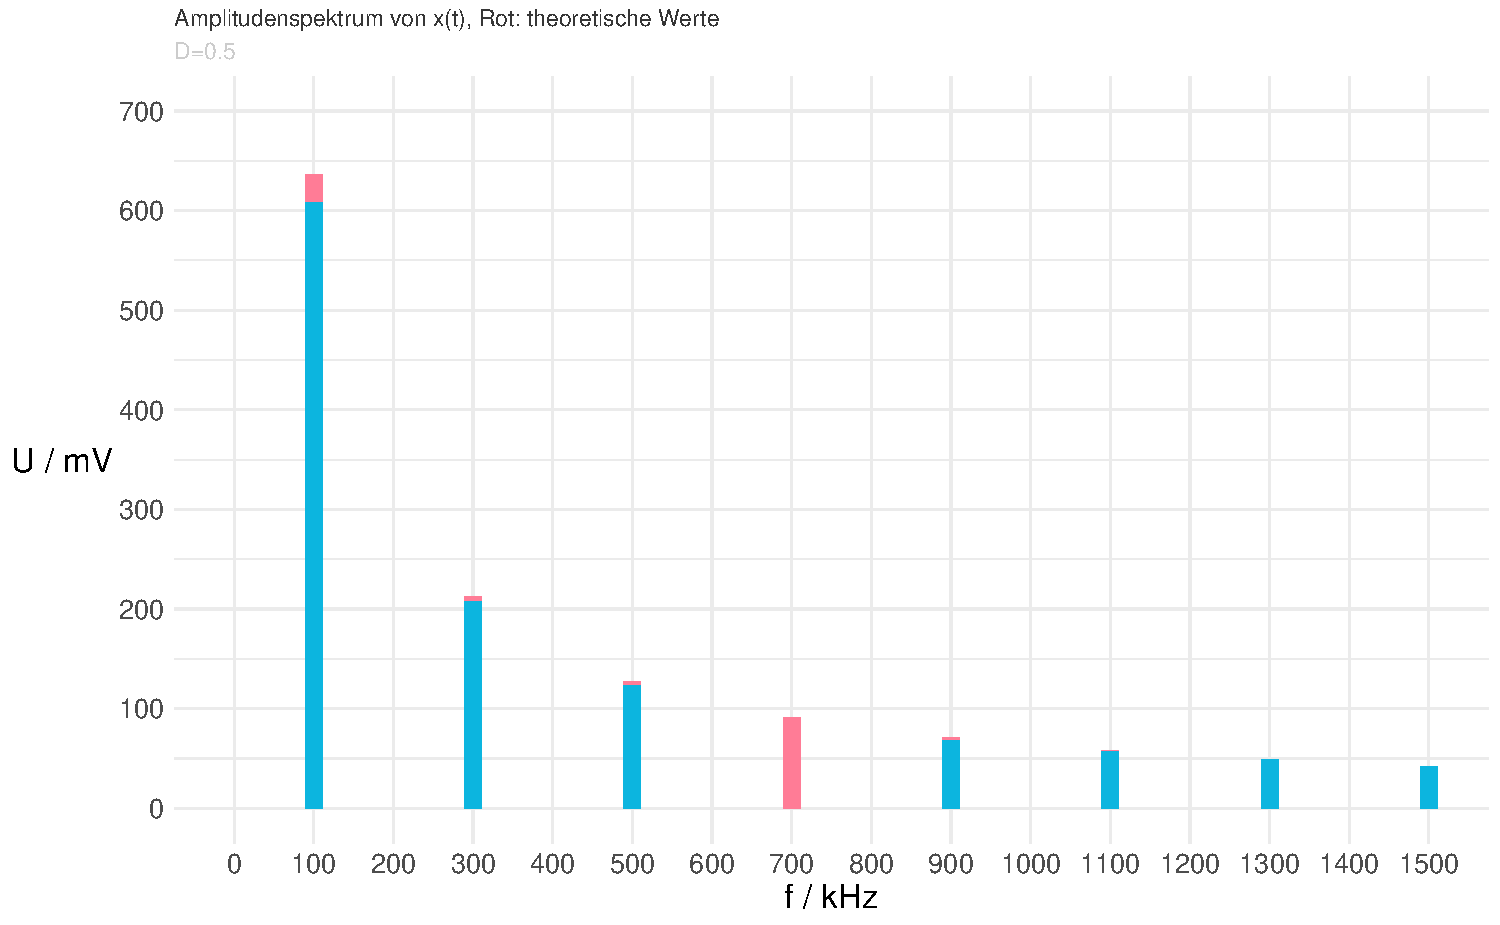
\includegraphics[scale=0.5]{./R/3_1/3_1_ASpektrum.pdf}
      \vspace{0.021276873\paperheight}
      \vspace{0.021276873\paperheight}
      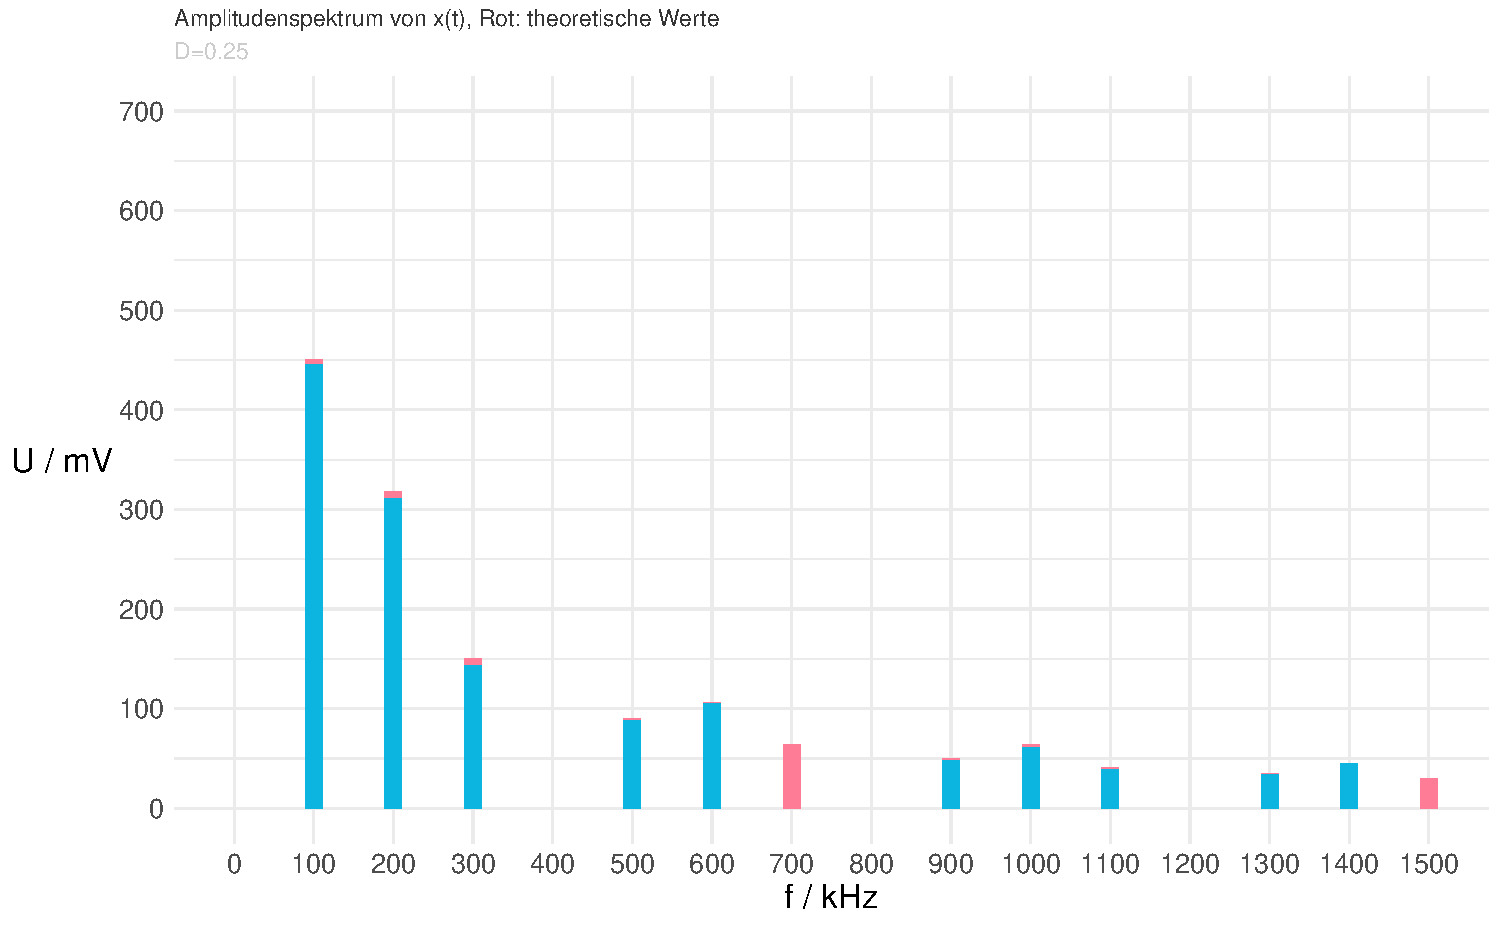
\includegraphics[scale=0.5]{./R/3_1/3_1_ASpektrum_025.pdf}
      \vspace{0.021276873\paperheight}
      \vspace{0.021276873\paperheight}
      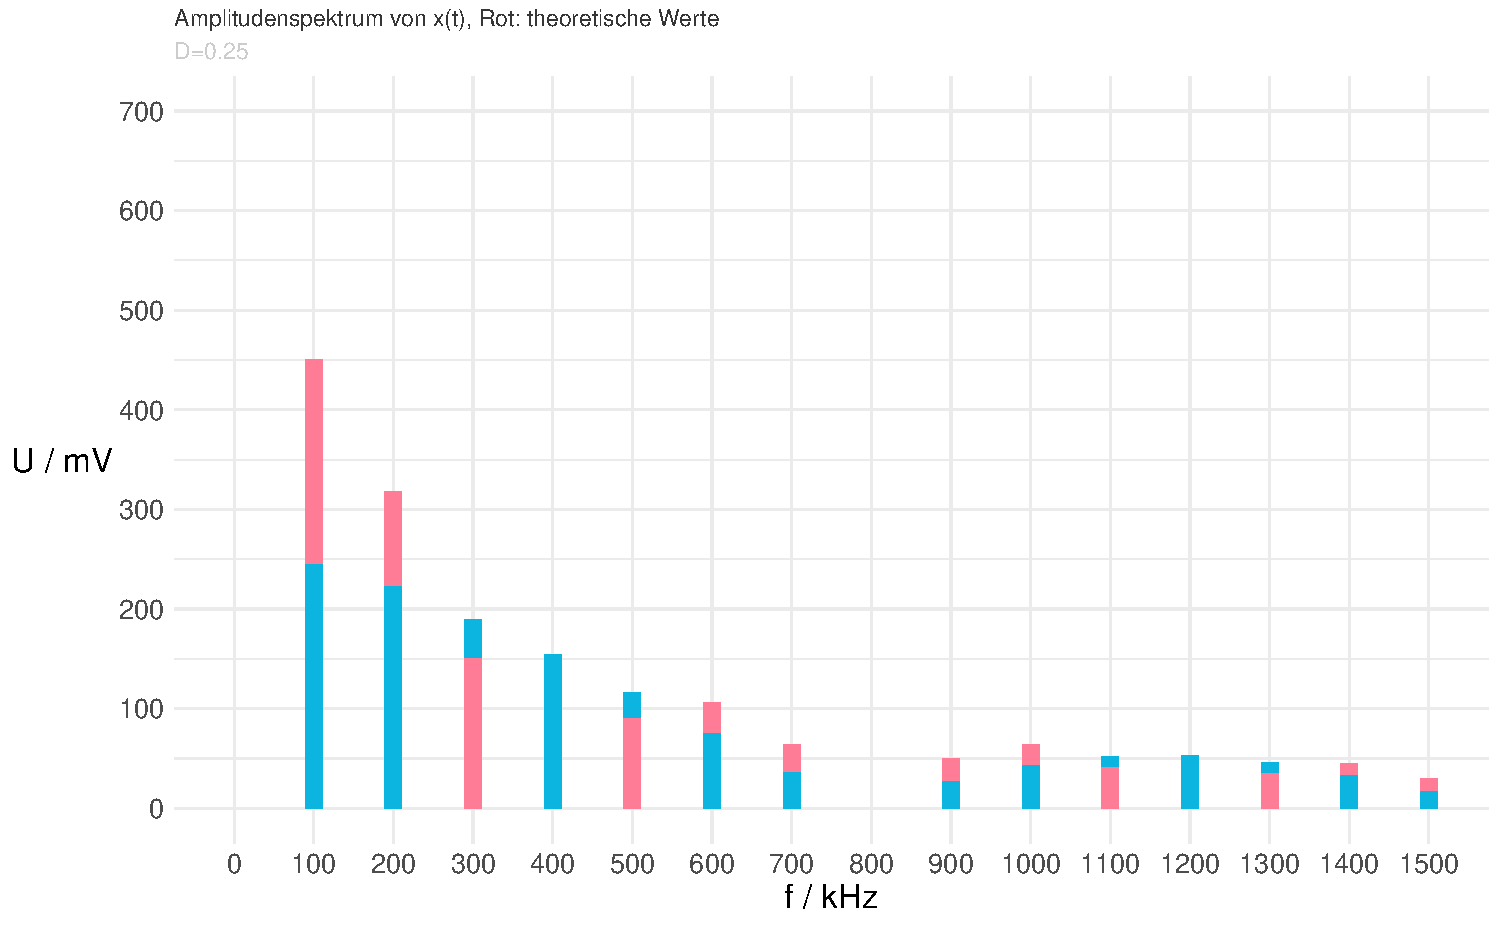
\includegraphics[scale=0.5]{./R/3_1/3_1_ASpektrum_0125.pdf}
    \end{center}


    \begin{center}
      \vspace{0.021276873\paperheight}
      \vspace{0.021276873\paperheight}

      Messwerte der Aufgabe 3.1 für \emph{$T=1 \,\ \si{\micro\second}$}:\\
      \vspace{0.021276873\paperheight}
      \bgroup
      \def\arraystretch{1.6180339887498948}
        \begin{tabular}{@{}cccc@{}}
        \toprule
        \multicolumn{3}{c}{$D = \frac{1}{2}, X_{\text{eff}}=692 \,\ \si{\milli\volt}$} \\ \midrule
        $\nu$      & $\hat{X}_\nu / \si{\milli\volt}$   & $X_{\nu_{\text{eff}}} / \si{\milli\volt}$ & $f_\nu / \si{\mega\hertz}$ \\ \hline
          1  & 627.911     & 444        & 1        \\
          2  & -           & -          & -        \\
          3  & 203.647     & 144        & 3        \\
          4  & -           & -          & -        \\
          5  & 119.077     & 84.2       & 5        \\
          6  & -           & -          & -        \\
          7  & 85.984      & 60.8       & 7        \\
          8  & -           & -          & -        \\
          9  & 63.922      & 45.2       & 9        \\
          10 & -           & -          & -        \\
          11 & 53.599      & 37.9       & 11       \\
          12 & -           & -          & -        \\
          13 & 46.528      & 32.9       & 13       \\
          14 & -           & -          & -        \\
          15 & 40.305      & 28.5       & 15       \\ \bottomrule
        \end{tabular}
        \egroup
        \vspace{0.021276873\paperheight}
        \bgroup
        \def\arraystretch{1.6180339887498948}
          \begin{tabular}{@{}cccc@{}}
          \toprule
          \multicolumn{3}{c}{$D = \frac{1}{4}, X_{\text{eff}}=489 \,\ \si{\milli\volt}$} \\ \midrule
          $\nu$      & $\hat{X}_\nu / \si{\milli\volt}$   & $X_{\nu_{\text{eff}}} / \si{\milli\volt}$ & $f_\nu / \si{\mega\hertz}$ \\ \hline
            1  & 445.477     & 315        & 1        \\
            2  & 308.864     & 218.4      & 2        \\
            3  & 143.401     & 101.4      & 3        \\
            4  & -           & -          & -        \\
            5  & 87.540      & 61.9       & 5        \\
            6  & 103.379     & 73.1       & 6        \\
            7  & 106.915     & 75.6       & 7        \\
            8  & -           & -          & -        \\
            9  & 47.800      & 33.8       & 9        \\
            10 & 59.256      & 41.9       & 10       \\
            11 & 38.467      & 27.2       & 11       \\
            12 & -           & -          & -        \\
            13 & 32.244      & 22.8       & 13       \\
            14 & 43.416      & 30.7       & 14       \\
            15 & 29.274      & 20.7       & 15       \\ \bottomrule
          \end{tabular}
          \egroup

          \bgroup
          \def\arraystretch{1.6180339887498948}
            \begin{tabular}{@{}cccc@{}}
            \toprule
            \multicolumn{3}{c}{$D = \frac{1}{10}, X_{\text{eff}} = 305 \,\ \si{\milli\volt}$} \\ \midrule
            $\nu$      & $\hat{X}_\nu / \si{\milli\volt}$   & $X_{\nu_{\text{eff}}} / \si{\milli\volt}$ & $f_\nu / \si{\mega\hertz}$ \\ \hline
              1  & 193.606     & 136.9      & 1        \\
              2  & 180.312     & 127.5      & 2        \\
              3  & 161.786     & 114.4      & 3        \\
              4  & 143.260     & 101.3      & 4        \\
              5  & 122.895     & 86.9       & 5        \\
              6  & 98.995      & 70         & 6        \\
              7  & 73.398      & 51.9       & 7        \\
              8  & 46.810      & 33.1       & 8        \\
              9  & 22.062      & 15.6       & 9        \\
              10 & -           & -          & -        \\
              11 & 15.415      & 10.9       & 11       \\
              12 & 28.426      & 20.1       & 12       \\
              13 & 37.052      & 26.2       & 13       \\
              14 & 40.871      & 28.9       & 14       \\
              15 & 39.881      & 28.2       & 15       \\ \bottomrule
            \end{tabular}
            \egroup
    \end{center}

    \begin{center}
      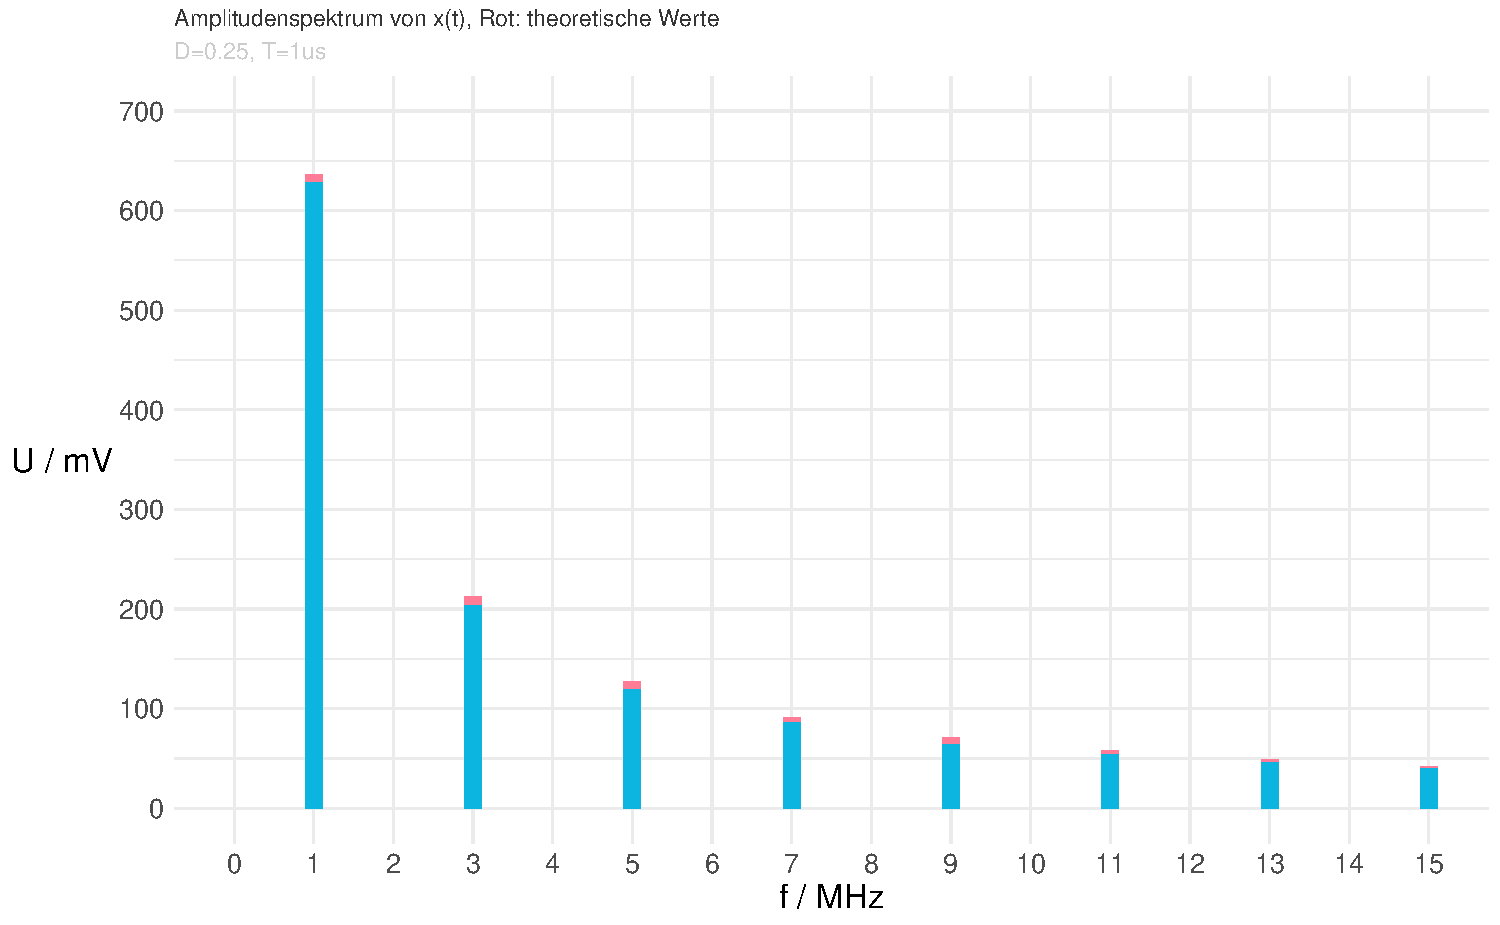
\includegraphics[scale=0.5]{./R/3_1/3_1_ASpektrum_05_2.pdf}
      \vspace{0.021276873\paperheight}
      \vspace{0.021276873\paperheight}
      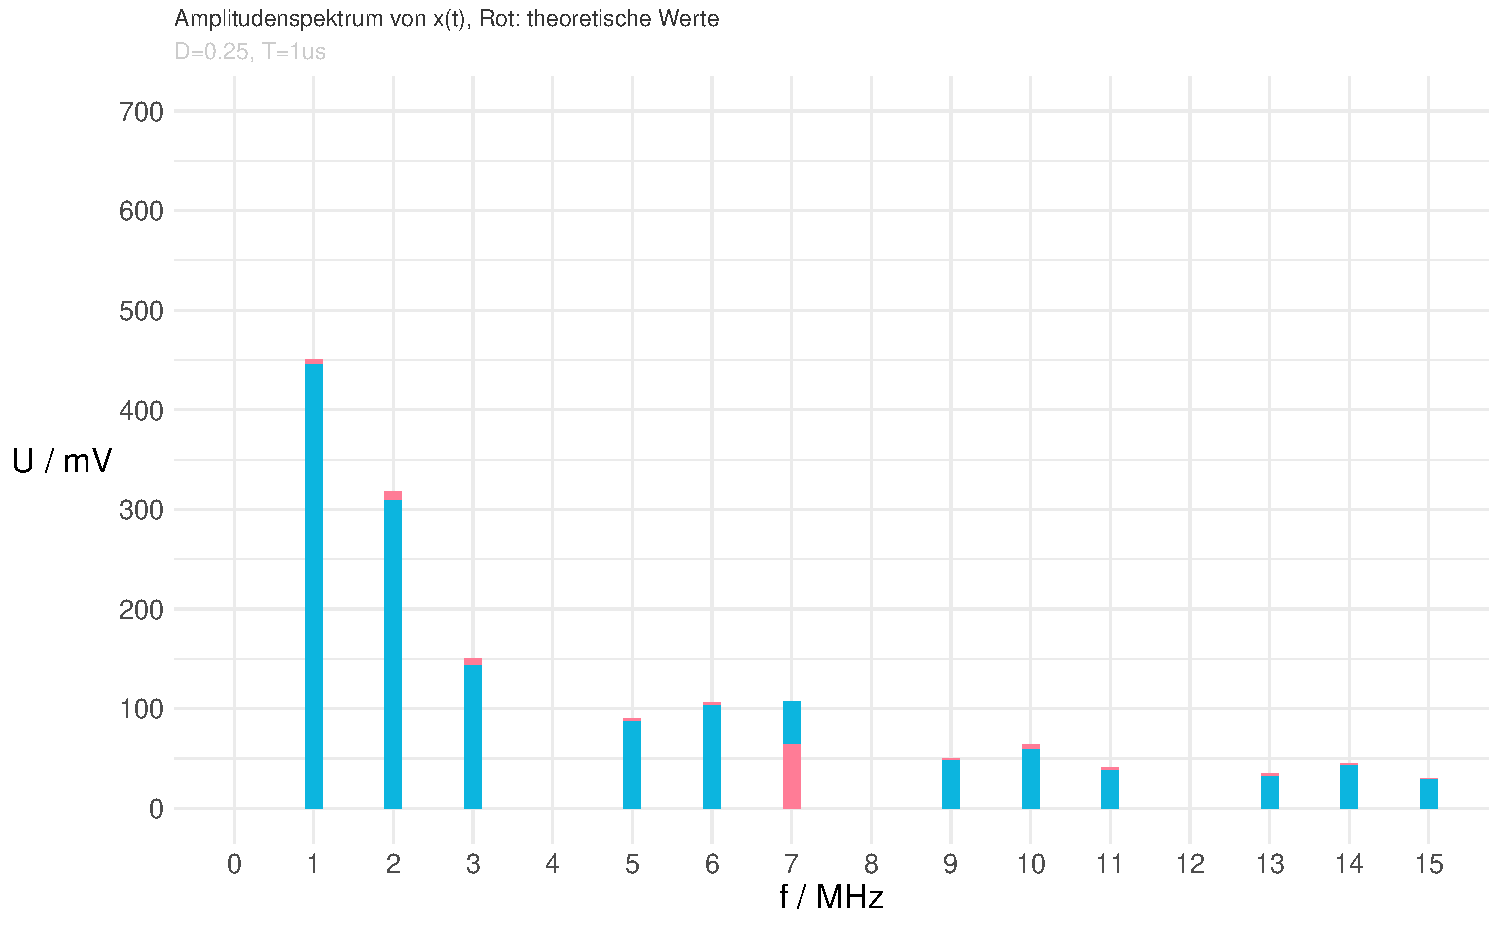
\includegraphics[scale=0.5]{./R/3_1/3_1_ASpektrum_025_2.pdf}
      \vspace{0.021276873\paperheight}
      \vspace{0.021276873\paperheight}
      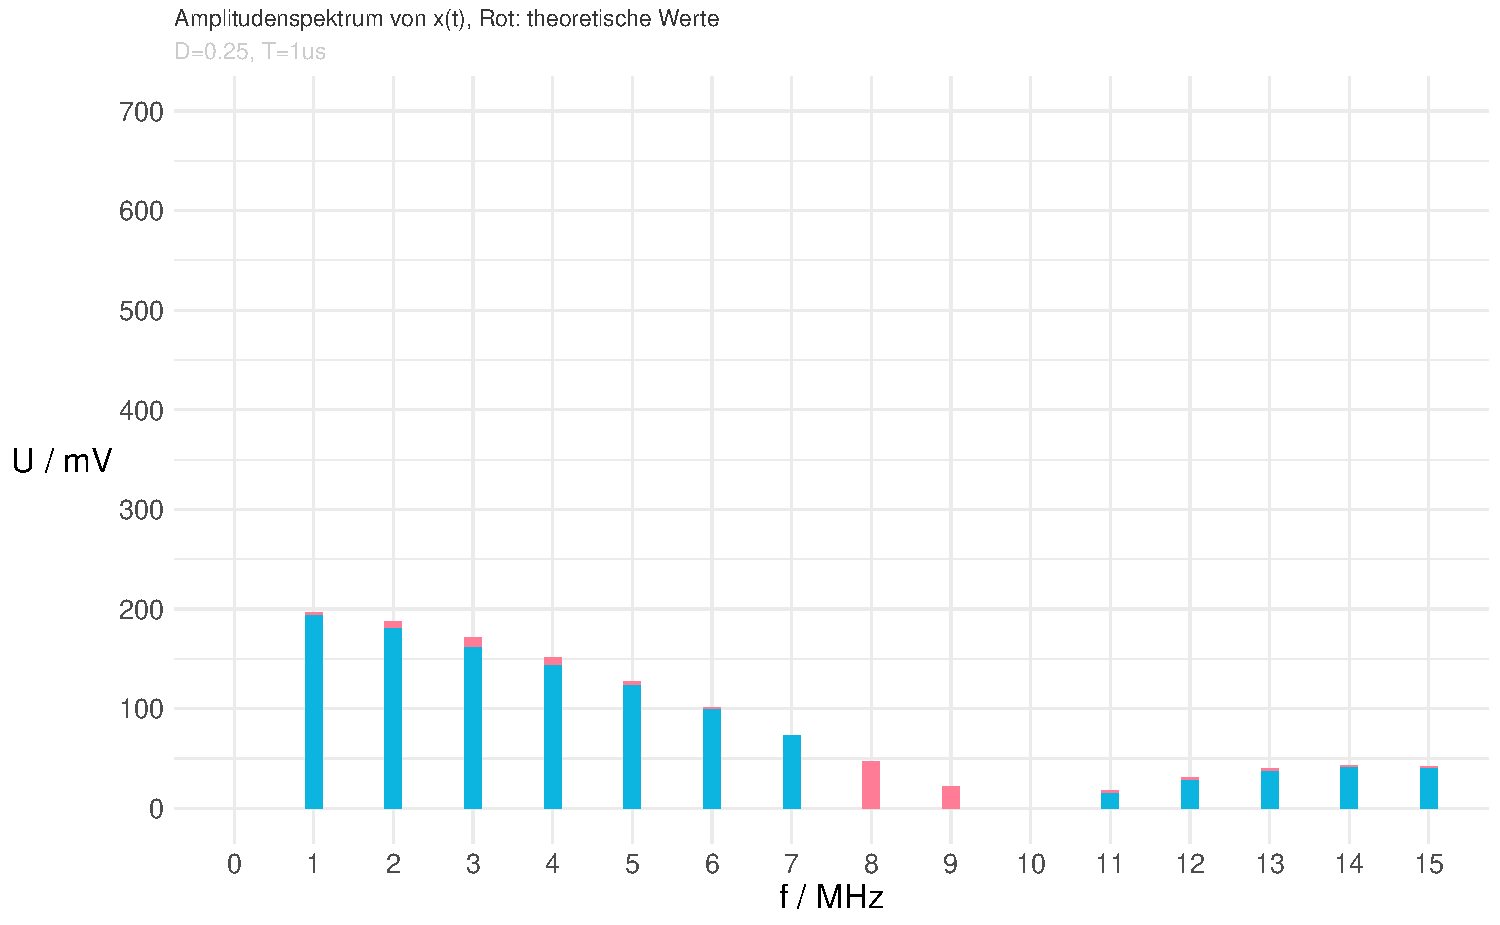
\includegraphics[scale=0.5]{./R/3_1/3_1_ASpektrum_01_2.pdf}
    \end{center}

  % 3.2
  \subsection{}
  \begin{center}
    \bgroup
    \def\arraystretch{1.6180339887498948}
      \begin{tabular}{@{}cccc@{}}
      \toprule
      \multicolumn{3}{c}{$X_{\text{eff}}=698
      \,\ \si{\milli\volt}, \,\ X_0 = 627 \,\ \si{\milli\volt}$} \\ \midrule
      $\nu$      & $\hat{X}_\nu / \si{\milli\volt}$   & $X_{\nu_{\text{eff}}} / \si{\milli\volt}$ & $f_\nu / \si{\kilo\hertz}$ \\ \hline
        1  & 406.021 & 287.1 & 1        \\
        2  & 85.843  & 60.7  & 2        \\
        3  & 39.881  & 28.2  & 3        \\
        4  & 23.617  & 16.7  & 4        \\
        5  & 17.395  & 12.3  & 5        \\
        6  & 13.011  & 9.2   & 6        \\
        7  & 9.475   & 6.7   & 7        \\
        8  & 8.202   & 5.8   & 8        \\
        9  & 6.930   & 4.9   & 9        \\
        10 & 5.940   & 4.2   & 10       \\
        11 & 4.808   & 3.4   & 11       \\
        12 & 4.384   & 3.1   & 12       \\
        13 & 4.243   & 3     & 13       \\
        14 & 3.536   & 2.5   & 14       \\
        15 & 3.253   & 2.3   & 15       \\
        16 & 2.828   & 2     & 16       \\ \bottomrule
      \end{tabular}\\
      Messwerte der Aufgabe 3.2\\
      \egroup
    \end{center}

    \begin{center}
      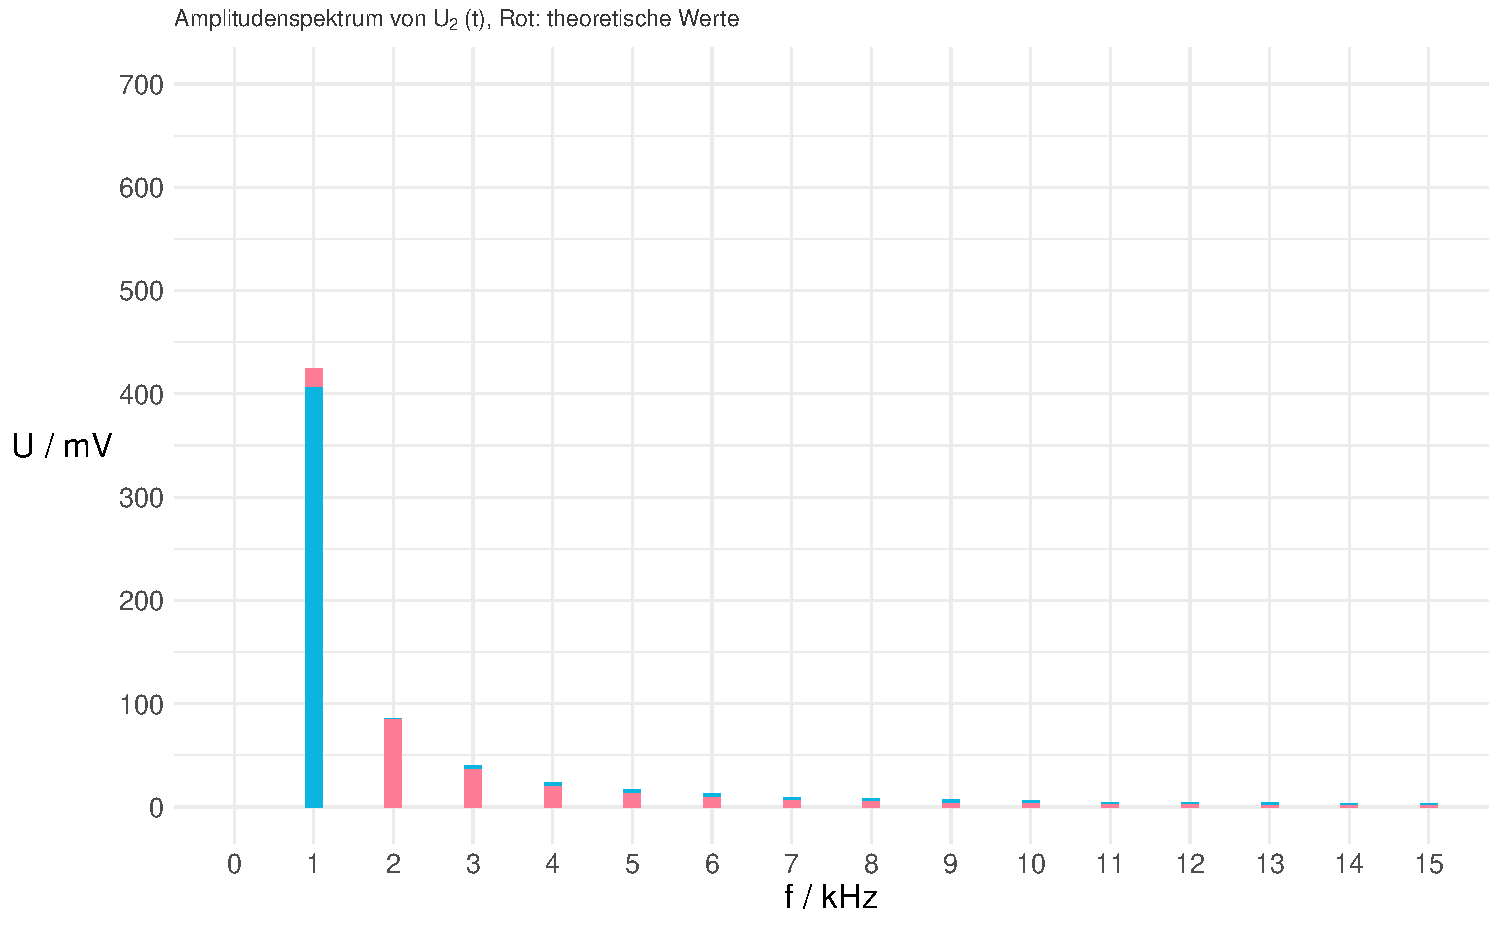
\includegraphics[scale=0.5]{./R/3_2/3_2_ASpektrum.pdf}
    \end{center}

  % 3.3
  \subsection{}

  \begin{center}
    \bgroup
    \def\arraystretch{1.6180339887498948}
      \begin{tabular}{@{}cccc@{}}
      \toprule
      \multicolumn{3}{c}{$U_{2_{\text{eff}}}=425
      \,\ \si{\milli\volt}, \,\ U_0 = 416 \,\ \si{\milli\volt}$} \\ \midrule
      $\nu$      & $\hat{X}_\nu / \si{\milli\volt}$   & $X_{\nu_{\text{eff}}} / \si{\milli\volt}$ & $f_\nu / \si{\kilo\hertz}$ \\ \hline
      1 & 117.238 & 82.9        & 1        \\
      2 & 12.445  & 8.8         & 2        \\
      3 & 3.677   & 2.6         & 3        \\
      4 & 1.485   & 1.05        & 4        \\
      5 & 0.813   & 0.575       & 5        \\
      6 & 0.443   & 0.313       & 6        \\
      7 & 0.252   & 0.178       & 7        \\
      8 & 0.208   & 0.147       & 8        \\ \bottomrule
      \end{tabular}\\
      Messwerte der Aufgabe 3.3\\
      \egroup
    \end{center}

  \begin{center}
    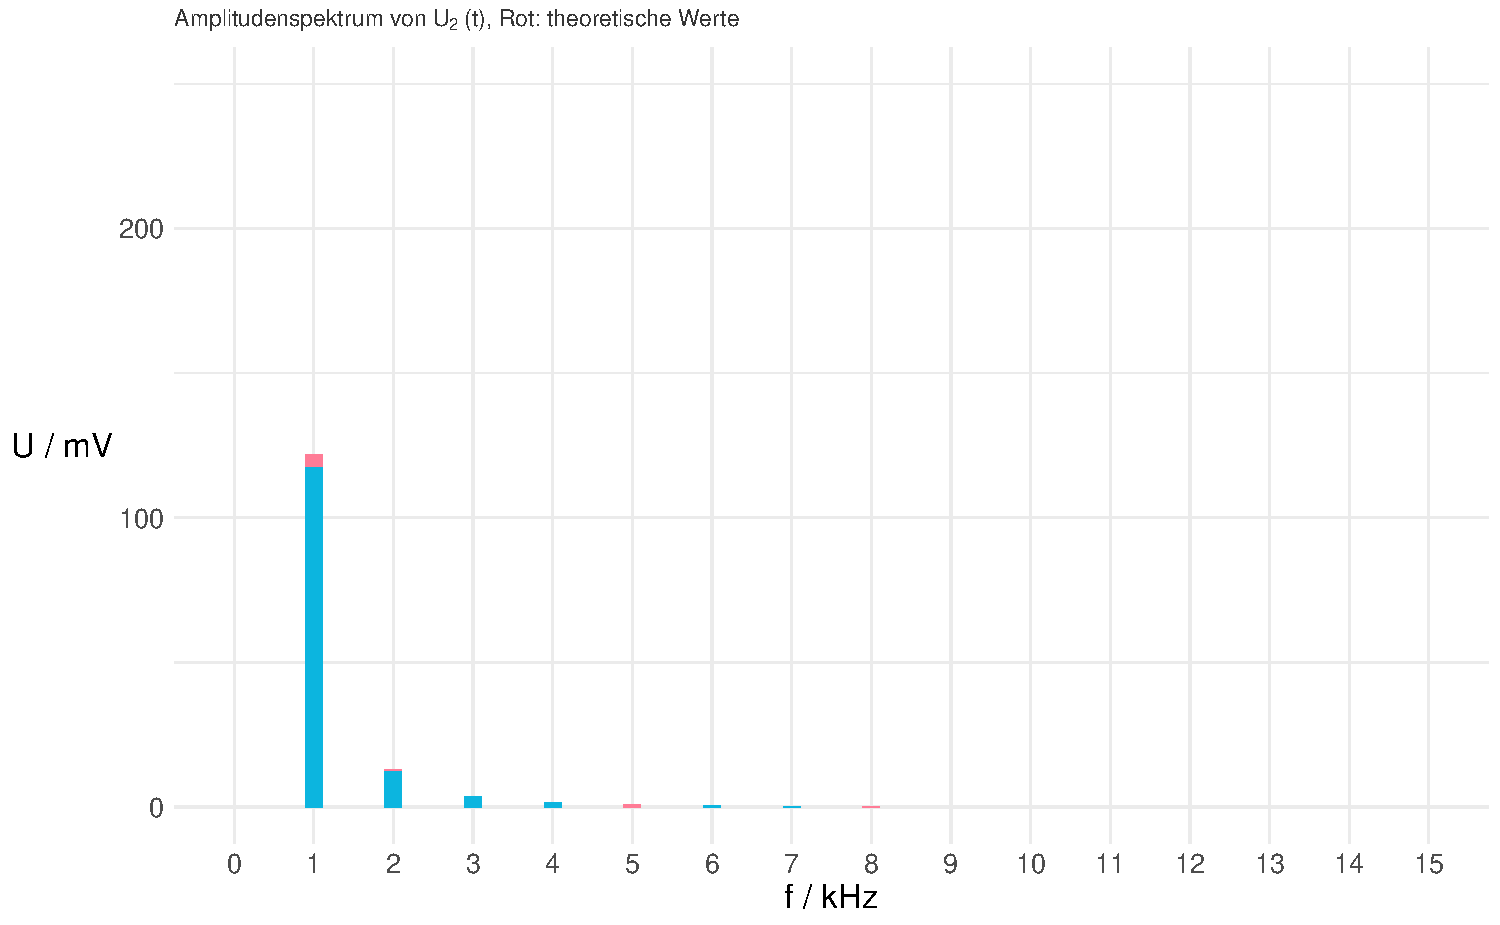
\includegraphics[scale=0.5]{./R/3_3/3_3_ASpektrum.pdf}
  \end{center}
  \vspace{0.021276873\paperheight}
  \begin{center}
    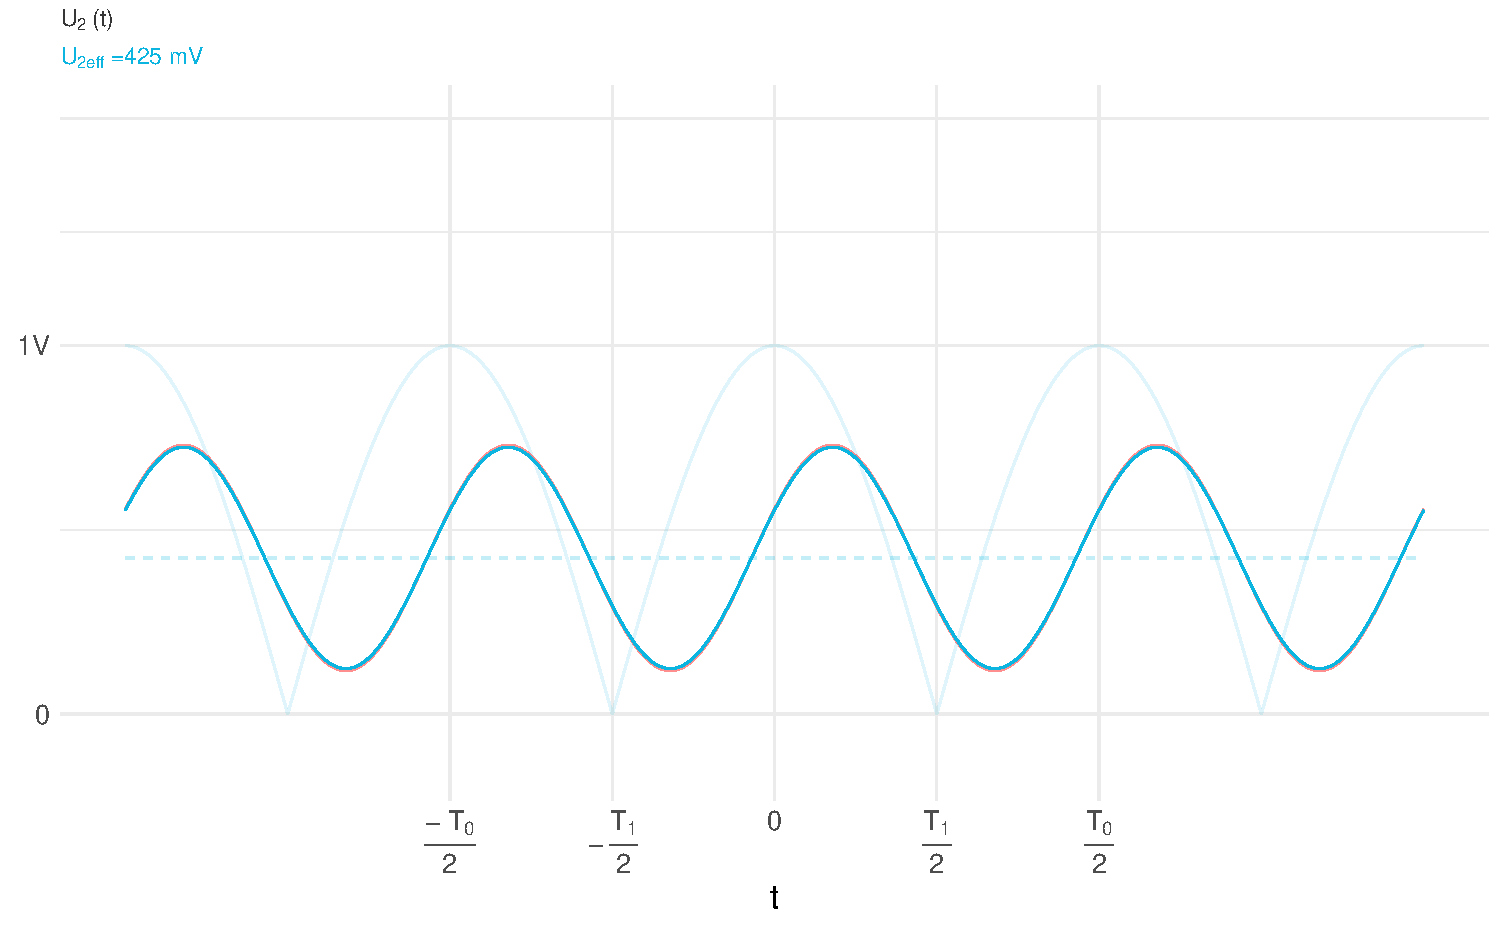
\includegraphics[scale=0.5]{./R/3_3/3_3_function.pdf}
  \end{center}


\end{document}
